\chapter{Fundamentos ecológicos do nicho}
%================================================

\begin{objetivos}
Ao final desta unidade, o estudante deverá ser capaz de:
\begin{itemize}
  \item compreender a base ecológica da Modelagem de Distribuição de Espécies (SDM) e da Modelagem de Nicho Ecológico (ENM);
  \item diferenciar os conceitos de nicho de Grinnell, Elton e Hutchinson;
  \item distinguir nicho fundamental, nicho realizado, distribuição observada e distribuição potencial;
  \item reconhecer o papel dos fatores abióticos, bióticos e históricos na distribuição das espécies;
  \item interpretar criticamente mapas de adequabilidade ambiental e projeções sob mudanças climáticas;
  \item compreender por que a conservação de nicho é uma hipótese central em projeções espaciais e temporais.
\end{itemize}
\end{objetivos}

\section{Introdução}

A Modelagem de Distribuição de Espécies, conhecida internacionalmente como \textit{Species Distribution Modeling} (SDM), \textit{Habitat Suitability Modeling} (HSM) ou \textit{Ecological Niche Modeling} (ENM), constitui uma das abordagens mais importantes da ecologia quantitativa contemporânea. Seu objetivo central é relacionar registros de ocorrência de uma espécie com condições ambientais observadas no espaço geográfico, permitindo estimar áreas ambientalmente adequadas à sua presença atual, passada ou futura \parencite{guisan2000,guisan2005predicting,guisan2017habitat,elith2009,franklin2010}.

Apesar de frequentemente ser apresentada como uma técnica computacional baseada em mapas, algoritmos e camadas ambientais, a SDM é, antes de tudo, uma aplicação ecológica do conceito de nicho. A qualidade de um modelo de distribuição depende não apenas da escolha do algoritmo, mas da coerência entre pergunta ecológica, dados de ocorrência, variáveis ambientais, escala espacial, área acessível, hipóteses biogeográficas e interpretação da adequabilidade ambiental \parencite{peterson2011,guisan2017habitat,barve2011crucial}.

Nesta unidade são apresentados os fundamentos ecológicos necessários para compreender o que os modelos de distribuição realmente estimam. Serão discutidos os conceitos clássicos de nicho de Grinnell, Elton e Hutchinson; a distinção entre nicho fundamental e nicho realizado; a diferença entre distribuição potencial e distribuição observada; e o papel da conservação de nicho em estudos de mudanças climáticas, invasões biológicas e conservação da biodiversidade.

\begin{conceito}
A SDM não deve ser entendida apenas como uma técnica de produção de mapas. Ela é uma estrutura de inferência ecológica que conecta ocorrências biológicas, espaço ambiental, espaço geográfico, hipóteses de nicho e decisões de conservação.
\end{conceito}

\section{Por que começar pelo conceito de nicho?}

Um erro comum em aplicações de SDM é iniciar a modelagem diretamente pelo software, pelos pacotes em R ou pelos algoritmos, sem definir previamente qual dimensão ecológica está sendo representada. No entanto, todo modelo de distribuição carrega uma hipótese sobre por que uma espécie ocorre em determinados locais e está ausente de outros.

De forma geral, a distribuição geográfica de uma espécie resulta da interação entre pelo menos três componentes principais: condições abióticas adequadas, interações bióticas favoráveis ou toleráveis e possibilidade histórica ou atual de dispersão até a área considerada. Essa lógica está no centro do chamado \textit{BAM framework}, no qual $B$ representa fatores bióticos, $A$ representa fatores abióticos e $M$ representa a área acessível por dispersão \parencite{soberon2005,soberon2009,barve2011crucial}.

Assim, uma espécie somente será observada em um local quando as condições ambientais estiverem dentro de seus limites de tolerância, quando as interações ecológicas não impedirem sua persistência e quando a espécie tiver conseguido alcançar aquele local ao longo de sua história evolutiva, biogeográfica ou demográfica.

\begin{equationbox}
\[
G_0 \approx A \cap B \cap M
\]
Em termos conceituais, a distribuição ocupada observável ($G_0$) tende a ocorrer na interseção entre condições abióticas adequadas ($A$), condições bióticas compatíveis ($B$) e área acessível à espécie ($M$).
\end{equationbox}

\begin{atencao}
Um modelo calibrado fora da área acessível ecologicamente plausível pode confundir ausência de dispersão com inadequação ambiental. Por isso, a delimitação da área de calibração é uma decisão ecológica, não apenas cartográfica.
\end{atencao}

\section{O nicho de Grinnell}

O conceito grinnelliano de nicho está associado principalmente aos requisitos ambientais que permitem a existência de uma espécie em determinada região. Nesse sentido, o nicho é entendido como o conjunto de condições físicas e climáticas necessárias para que uma população sobreviva e se mantenha ao longo do tempo \parencite{grinnell1917,soberon2007}.

Esse conceito é particularmente importante para SDM porque muitos modelos utilizam variáveis climáticas, topográficas e edáficas como preditoras da distribuição das espécies. Quando usamos temperatura média anual, precipitação, sazonalidade climática, altitude, declividade, textura do solo ou déficit hídrico climático, estamos trabalhando predominantemente com uma interpretação grinnelliana do nicho.

Em escalas amplas, como continentes, biomas ou grandes regiões hidroclimáticas, fatores climáticos tendem a exercer forte controle sobre os limites de distribuição das espécies. Por isso, modelos baseados em variáveis bioclimáticas são frequentemente aplicados para prever distribuição potencial, mudanças futuras de área adequada e deslocamentos de faixa climática sob cenários de mudanças climáticas \parencite{guisan2005predicting,elith2009,guisan2017habitat}.

\begin{dica}[title={\faLightbulb\quad dica}]
Em SDM, variáveis grinnellianas são especialmente úteis quando a pergunta envolve macroecologia, biogeografia, mudanças climáticas, invasões biológicas ou conservação em grandes escalas espaciais.
\end{dica}

\section{O nicho de Elton}

O conceito eltoniano de nicho enfatiza o papel funcional da espécie na comunidade ecológica. Diferentemente da visão grinnelliana, centrada nos requisitos ambientais, o nicho eltoniano destaca o que a espécie faz no ecossistema: suas interações tróficas, seus recursos alimentares, seus predadores, seus competidores, seus mutualistas e seus efeitos sobre outras espécies \parencite{elton1927,soberon2007}.

Em termos práticos, o nicho de Elton está relacionado à posição da espécie na rede de interações ecológicas. Para plantas, isso pode incluir relações com polinizadores, dispersores, fungos micorrízicos, herbívoros, patógenos, competidores por luz, água e nutrientes. Para animais, pode envolver dieta, comportamento de forrageamento, predação, parasitismo e relações de dependência com habitats ou espécies-chave.

Embora essencial para a compreensão ecológica completa da distribuição das espécies, o nicho eltoniano é mais difícil de incorporar em SDM tradicionais. Isso ocorre porque dados espacialmente explícitos sobre interações bióticas raramente estão disponíveis na mesma extensão, resolução e qualidade dos dados climáticos. Por isso, muitos modelos acabam representando principalmente o componente abiótico da distribuição, enquanto as interações bióticas permanecem implícitas, ausentes ou apenas parcialmente representadas.

\begin{atencao}[title={\faExclamationTriangle\quad atenção}]
A ausência de variáveis bióticas em um SDM não significa que interações ecológicas sejam irrelevantes. Significa apenas que, em muitos casos, elas não foram medidas ou não estão disponíveis em resolução compatível com a análise.
\end{atencao}

\section{O nicho de Hutchinson}

O conceito de nicho de Hutchinson representa uma das formulações mais influentes da ecologia moderna. Hutchinson definiu o nicho como um hipervolume $n$-dimensional, no qual cada dimensão representa uma variável ambiental ou ecológica relevante para a persistência da espécie. Dentro desse hipervolume, as condições permitem crescimento populacional positivo; fora dele, a população não consegue se manter ao longo do tempo \parencite{hutchinson1957,colwell2009}.

Essa definição é fundamental para SDM porque permite separar o espaço geográfico do espaço ambiental. O espaço geográfico corresponde às coordenadas, mapas e regiões onde a espécie pode ocorrer. O espaço ambiental corresponde aos valores das variáveis que caracterizam os locais, como temperatura, precipitação, altitude, solo, sazonalidade e disponibilidade hídrica.

A modelagem de distribuição opera justamente nessa relação entre espaço ambiental e espaço geográfico. Primeiro, os registros de ocorrência são associados às condições ambientais dos locais onde a espécie foi observada. Em seguida, o modelo estima a resposta da espécie nesse espaço ambiental. Por fim, essa resposta é projetada de volta para o espaço geográfico, gerando mapas de adequabilidade ambiental \parencite{guisan2017habitat,raes2018modeling}.

\begin{conceito}
O espaço geográfico é o mapa: coordenadas, pixels, polígonos, bacias, biomas e unidades de conservação. O espaço ambiental é o conjunto de condições associadas a cada local: temperatura, precipitação, solo, altitude, sazonalidade, déficit hídrico e outras variáveis. A SDM aprende padrões no espaço ambiental e projeta esses padrões no espaço geográfico.
\end{conceito}

\section{Nicho fundamental e nicho realizado}

O nicho fundamental corresponde ao conjunto de condições ambientais sob as quais uma espécie poderia manter populações viáveis na ausência de restrições bióticas negativas e barreiras de dispersão. Em outras palavras, representa o espaço de tolerância fisiológica e ecológica potencial da espécie \parencite{hutchinson1957,pulliam2000,soberon2005}.

O nicho realizado é a porção do nicho fundamental efetivamente ocupada pela espécie sob condições naturais. Ele resulta da combinação entre tolerâncias ambientais, interações bióticas, dispersão, história evolutiva, filtros regionais e disponibilidade real de ambientes \parencite{pulliam2000,soberon2009}.

Na prática, o nicho fundamental raramente é estimado diretamente por SDM correlativos baseados em ocorrências naturais. Isso ocorre porque os registros de campo já refletem restrições de dispersão, história biogeográfica, interações ecológicas, filtros ambientais atuais e limitações amostrais. Assim, modelos baseados apenas em ocorrências geralmente estimam uma aproximação do nicho realizado ou de parte dele, não o nicho fundamental completo.

\begin{atencao}
Modelos correlativos inferem associações entre ocorrência e ambiente. Eles não medem diretamente taxa de crescimento populacional, sobrevivência, fecundidade, mortalidade, condutância estomática, vulnerabilidade hidráulica ou tolerância térmica. Para aproximar o nicho fundamental, são necessários dados experimentais, fisiológicos, demográficos ou modelos mecanísticos.
\end{atencao}

\section{Distribuição observada, real e potencial}

A distribuição observada corresponde aos registros conhecidos da espécie. Esses registros podem vir de herbários, museus, inventários florestais, bases de dados de biodiversidade, literatura científica, coleções biológicas, levantamentos de campo ou monitoramentos sistemáticos. Embora sejam a base dos modelos, os dados de ocorrência raramente representam perfeitamente a distribuição real da espécie \parencite{hijmans2021,guisan2017habitat}.

A distribuição real corresponde ao conjunto de locais efetivamente ocupados pela espécie em determinado período, independentemente de terem sido amostrados. Já a distribuição potencial representa o conjunto de áreas que apresentam condições ambientais adequadas para a espécie, de acordo com o modelo ajustado.

\begin{conceito}
A distribuição observada é uma amostra dos registros conhecidos; a distribuição real é a ocupação efetiva da espécie na paisagem; e a distribuição potencial é a projeção espacial das condições estimadas como adequadas pelo modelo.
\end{conceito}

Em espécies amazônicas, esse problema é especialmente relevante, pois grandes regiões permanecem subamostradas, o acesso é difícil e muitos registros estão concentrados próximos a rios, estradas, cidades, unidades de pesquisa e áreas historicamente mais inventariadas. Assim, ausência de registros não deve ser automaticamente interpretada como ausência ecológica.

\begin{dica}
Prefira interpretar mapas contínuos de adequabilidade como gradientes de suporte ambiental ao modelo, e não como mapas absolutos de presença e ausência. A transformação em mapas binários pode ser útil para algumas aplicações, mas sempre depende da escolha de limiares, que introduzem novas decisões metodológicas e incertezas.
\end{dica}

\section{Conservação de nicho}

A conservação de nicho refere-se à tendência de uma espécie ou linhagem manter, ao longo do tempo evolutivo ou entre regiões, requisitos ambientais semelhantes aos de seus ancestrais ou populações de origem. Esse conceito é central em estudos de mudanças climáticas, invasões biológicas, biogeografia histórica e projeções futuras de distribuição \parencite{peterson2011,guisan2017habitat,raes2018modeling}.

Quando projetamos um modelo calibrado no presente para o futuro, assumimos que a relação entre a espécie e o ambiente será suficientemente conservada para permitir inferência. Da mesma forma, quando usamos ocorrências da área nativa para prever o potencial invasivo em outra região, assumimos que a espécie manterá parte importante de seu nicho climático.

No entanto, a conservação de nicho não deve ser tratada como regra absoluta. Nichos podem se expandir, contrair ou mudar entre regiões e períodos. Mudanças aparentes podem resultar de evolução adaptativa, plasticidade fenotípica, liberação de inimigos naturais, novas interações ecológicas, ausência de competidores, mudanças na disponibilidade ambiental ou diferenças na amostragem.

\begin{atencao}
Projetar não é prever com certeza. Projeções futuras de SDM representam cenários condicionais: se a relação estimada entre ocorrência e ambiente permanecer válida, se as variáveis escolhidas forem relevantes, se o cenário climático ocorrer, e se dispersão e interações não impedirem a ocupação, então determinadas áreas poderão se tornar mais ou menos adequadas.
\end{atencao}

\section{Relação entre nicho e mudanças climáticas}

As mudanças climáticas modificam a distribuição espacial das condições ambientais que compõem o nicho das espécies. À medida que temperatura, precipitação, sazonalidade, déficit hídrico e frequência de extremos se alteram, áreas atualmente adequadas podem se tornar inadequadas, enquanto novas áreas podem se tornar ambientalmente compatíveis.

Em regiões tropicais, especialmente na Amazônia, mudanças no regime de chuvas, aumento da temperatura, intensificação do déficit de pressão de vapor, secas extremas e eventos associados ao El Niño podem alterar profundamente os filtros ambientais que estruturam a distribuição das espécies arbóreas. Para árvores gigantes, essas mudanças podem ser ainda mais críticas, pois indivíduos de grande porte dependem de estabilidade hidráulica, solos profundos, acesso contínuo à água e resistência mecânica a eventos extremos.

\begin{aplicacao}
Em estudos sobre árvores gigantes da Amazônia, a distribuição atual de indivíduos adultos pode refletir décadas ou séculos de condições ambientais favoráveis. Portanto, modelos baseados apenas em presença de adultos podem capturar a adequabilidade histórica para sobrevivência, mas não necessariamente a adequabilidade atual para regeneração. Uma abordagem robusta deve considerar, sempre que possível, diferentes estágios ontogenéticos, estrutura florestal, clima extremo, solo, hidrologia e estabilidade da paisagem.
\end{aplicacao}

\section{Síntese conceitual da unidade}

A modelagem de distribuição de espécies é uma ferramenta poderosa, mas sua interpretação depende de fundamentos ecológicos sólidos. O nicho de Grinnell orienta a relação entre espécie e ambiente físico; o nicho de Elton destaca o papel das interações ecológicas; e o nicho de Hutchinson fornece a base formal para compreender o nicho como um hipervolume multidimensional.

O nicho fundamental representa o conjunto de condições potencialmente toleradas pela espécie, enquanto o nicho realizado corresponde à porção efetivamente ocupada sob restrições bióticas, históricas, ambientais e de dispersão. A distribuição observada é uma amostra geográfica imperfeita dos locais conhecidos de ocorrência, enquanto a distribuição potencial representa a projeção espacial das condições estimadas como adequadas pelo modelo.

\begin{leitura}
Para aprofundamento conceitual, recomenda-se iniciar por \textcite{guisan2005predicting}, \textcite{soberon2007}, \textcite{soberon2009}, \textcite{peterson2011} e \textcite{guisan2017habitat}. Esses trabalhos formam a base conceitual moderna para interpretar nichos ecológicos, áreas de distribuição, adequabilidade ambiental e projeções espaço-temporais.
\end{leitura}

\subsection{Estudo de caso real: nicho ecológico climático de \textit{Dinizia excelsa}}

Nesta etapa, a simulação didática inicial é substituída por um estudo de caso real com registros de ocorrência de \textit{Dinizia excelsa} no bioma Amazônia. A espécie é uma árvore amazônica de grande porte, com importância ecológica, estrutural e conservacionista, sendo adequada para demonstrar como dados reais de ocorrência podem ser integrados a variáveis ambientais em uma análise inicial de nicho ecológico.

O objetivo desta unidade não é ainda ajustar um modelo preditivo completo, mas representar o espaço ambiental ocupado pela espécie em relação ao conjunto de condições climáticas disponíveis no bioma Amazônia. Para isso, os registros corrigidos de ocorrência foram filtrados espacialmente pelo limite do bioma e associados a variáveis bioclimáticas atuais derivadas do WorldClim.

Foram utilizadas quatro variáveis ambientais selecionadas: temperatura média anual, sazonalidade da temperatura, precipitação anual e sazonalidade da precipitação. Essas variáveis representam gradientes climáticos amplos associados ao nicho grinnelliano da espécie, isto é, ao conjunto de condições ambientais que podem favorecer, limitar ou restringir sua ocorrência geográfica.

\rscriptfile{scripts/unidade01/01_simulacao_nicho_ecologico.R}

\begin{figure}[H]
	\centering
	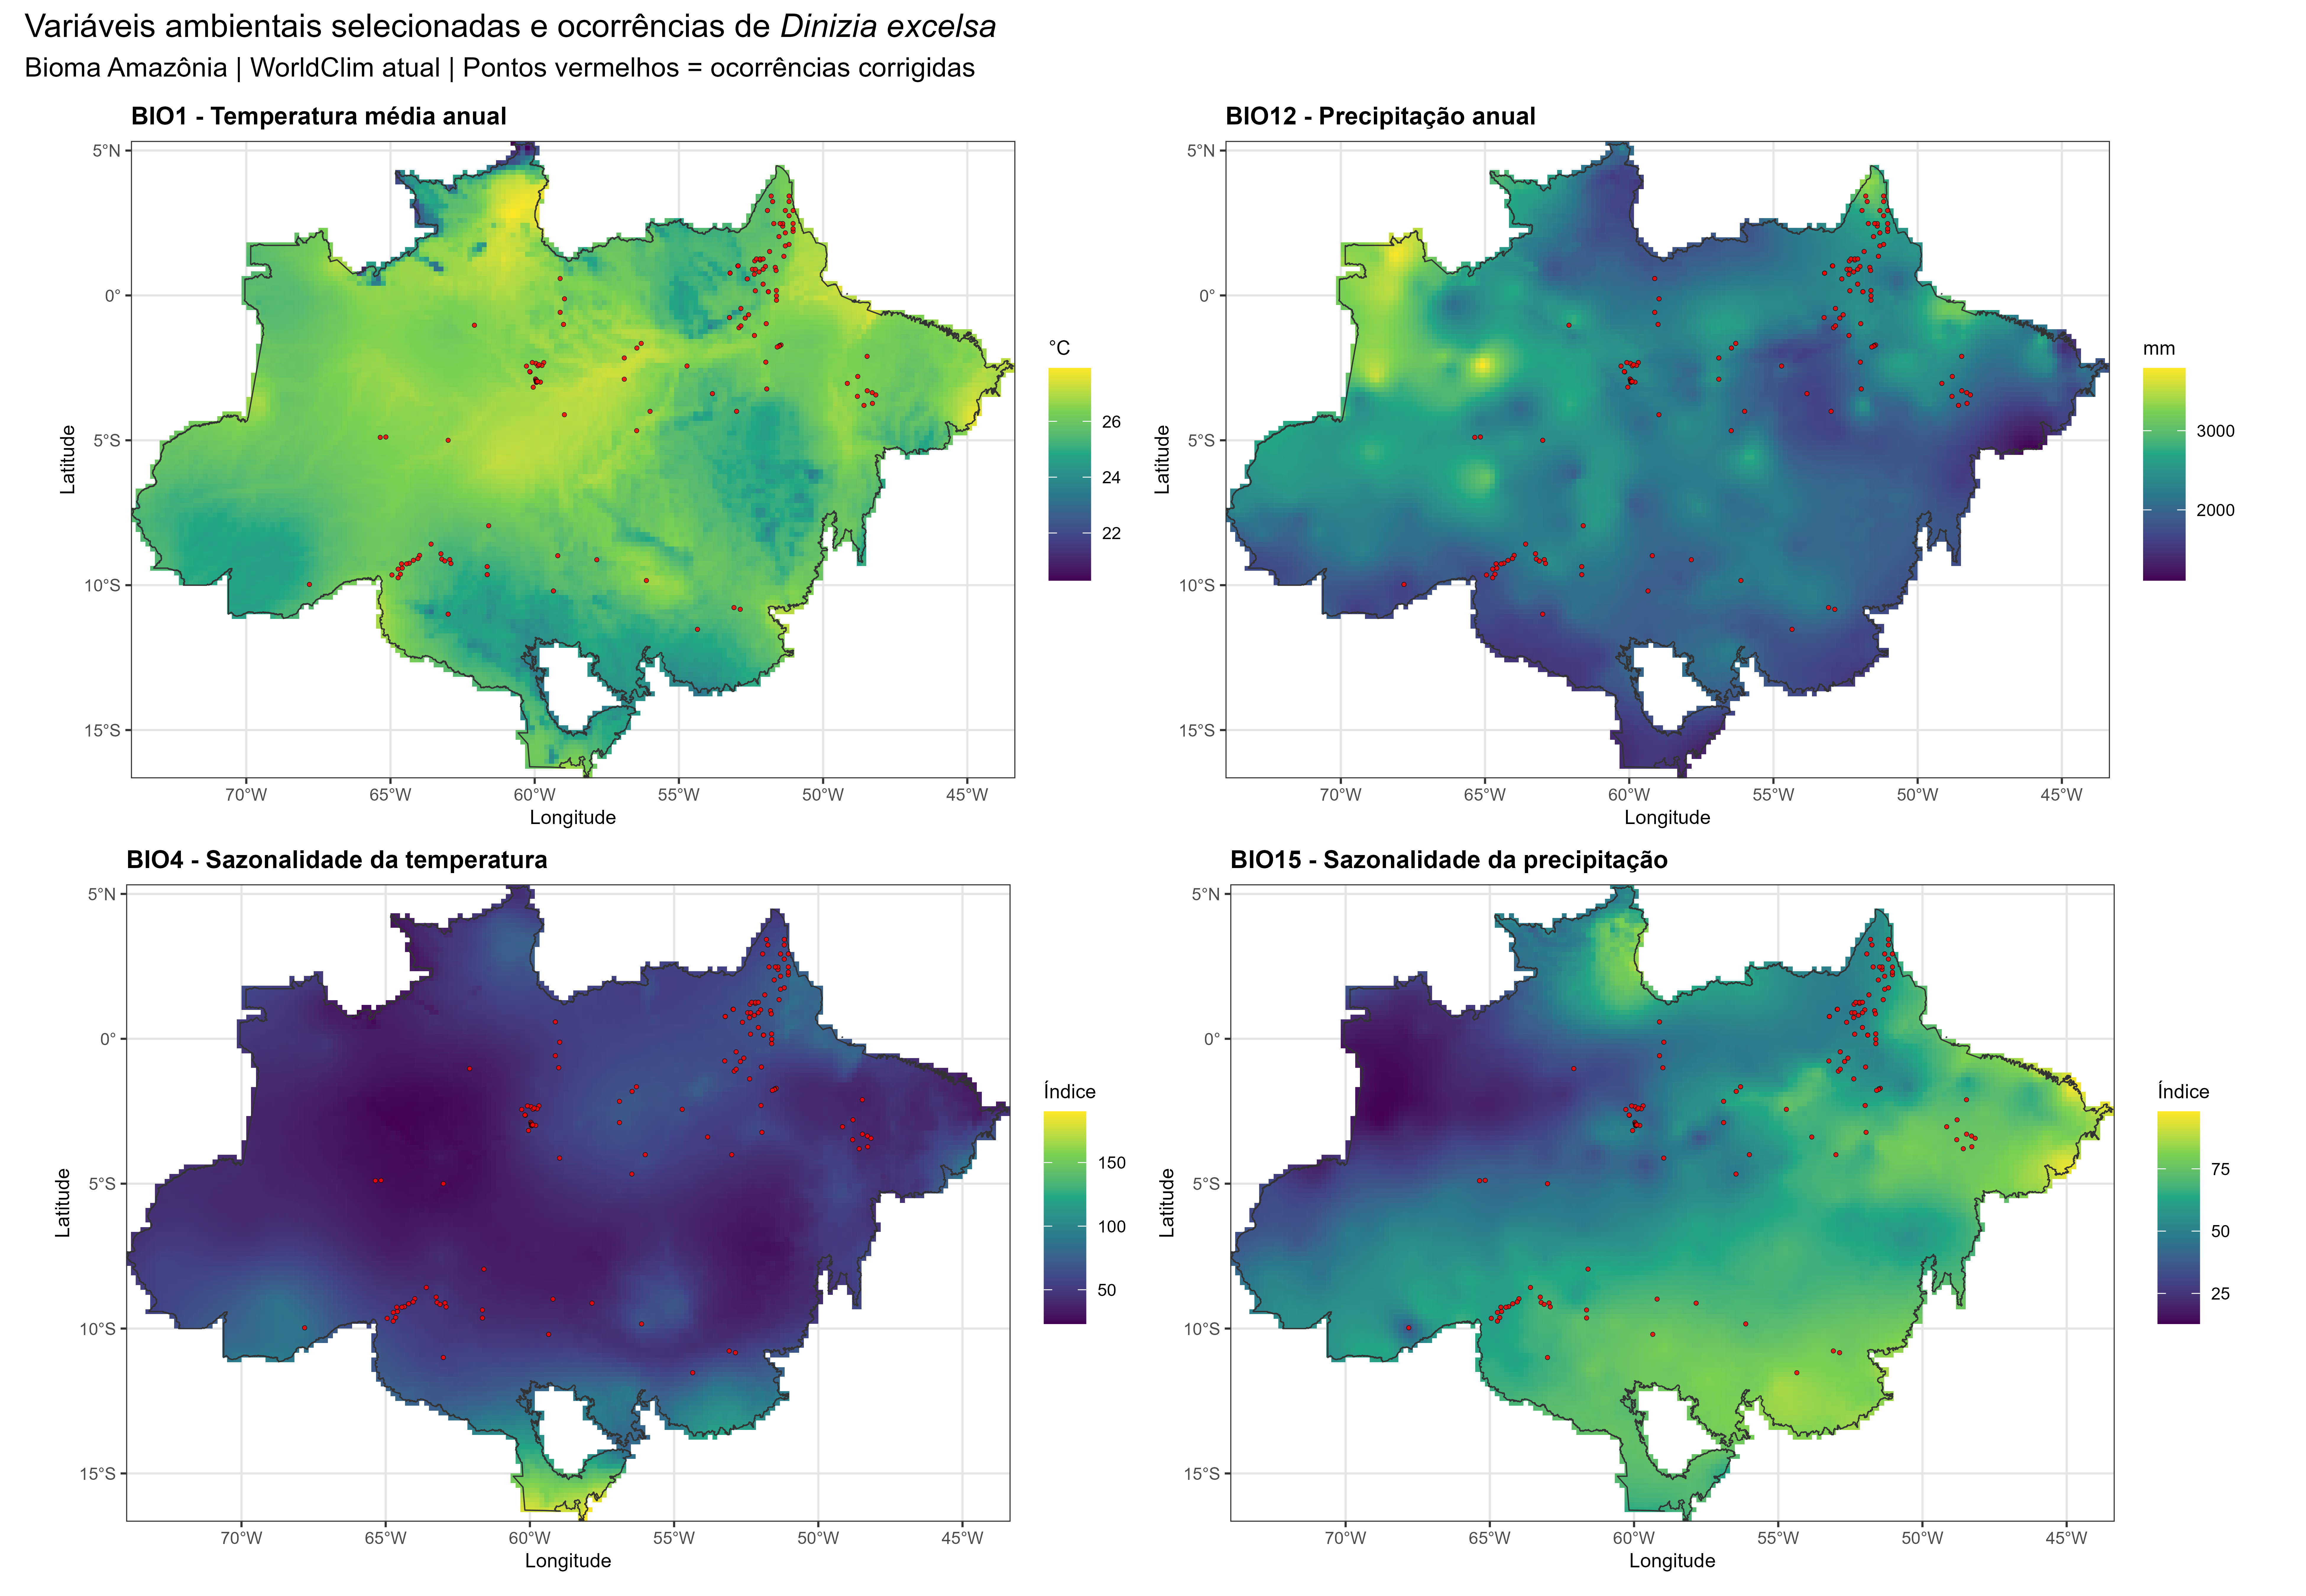
\includegraphics[width=0.96\textwidth]{figuras/unidade01/unidade01_mapas_variaveis_patchwork_dinizia.png}
	\caption{Variáveis ambientais selecionadas no bioma Amazônia com registros corrigidos de \textit{Dinizia excelsa}. Cada painel possui escala própria de cores, permitindo visualizar adequadamente a distribuição espacial de temperatura média anual, sazonalidade da temperatura, precipitação anual e sazonalidade da precipitação.}
	\label{fig:unidade01_variaveis_patchwork_dinizia}
\end{figure}

\begin{figure}[H]
	\centering
	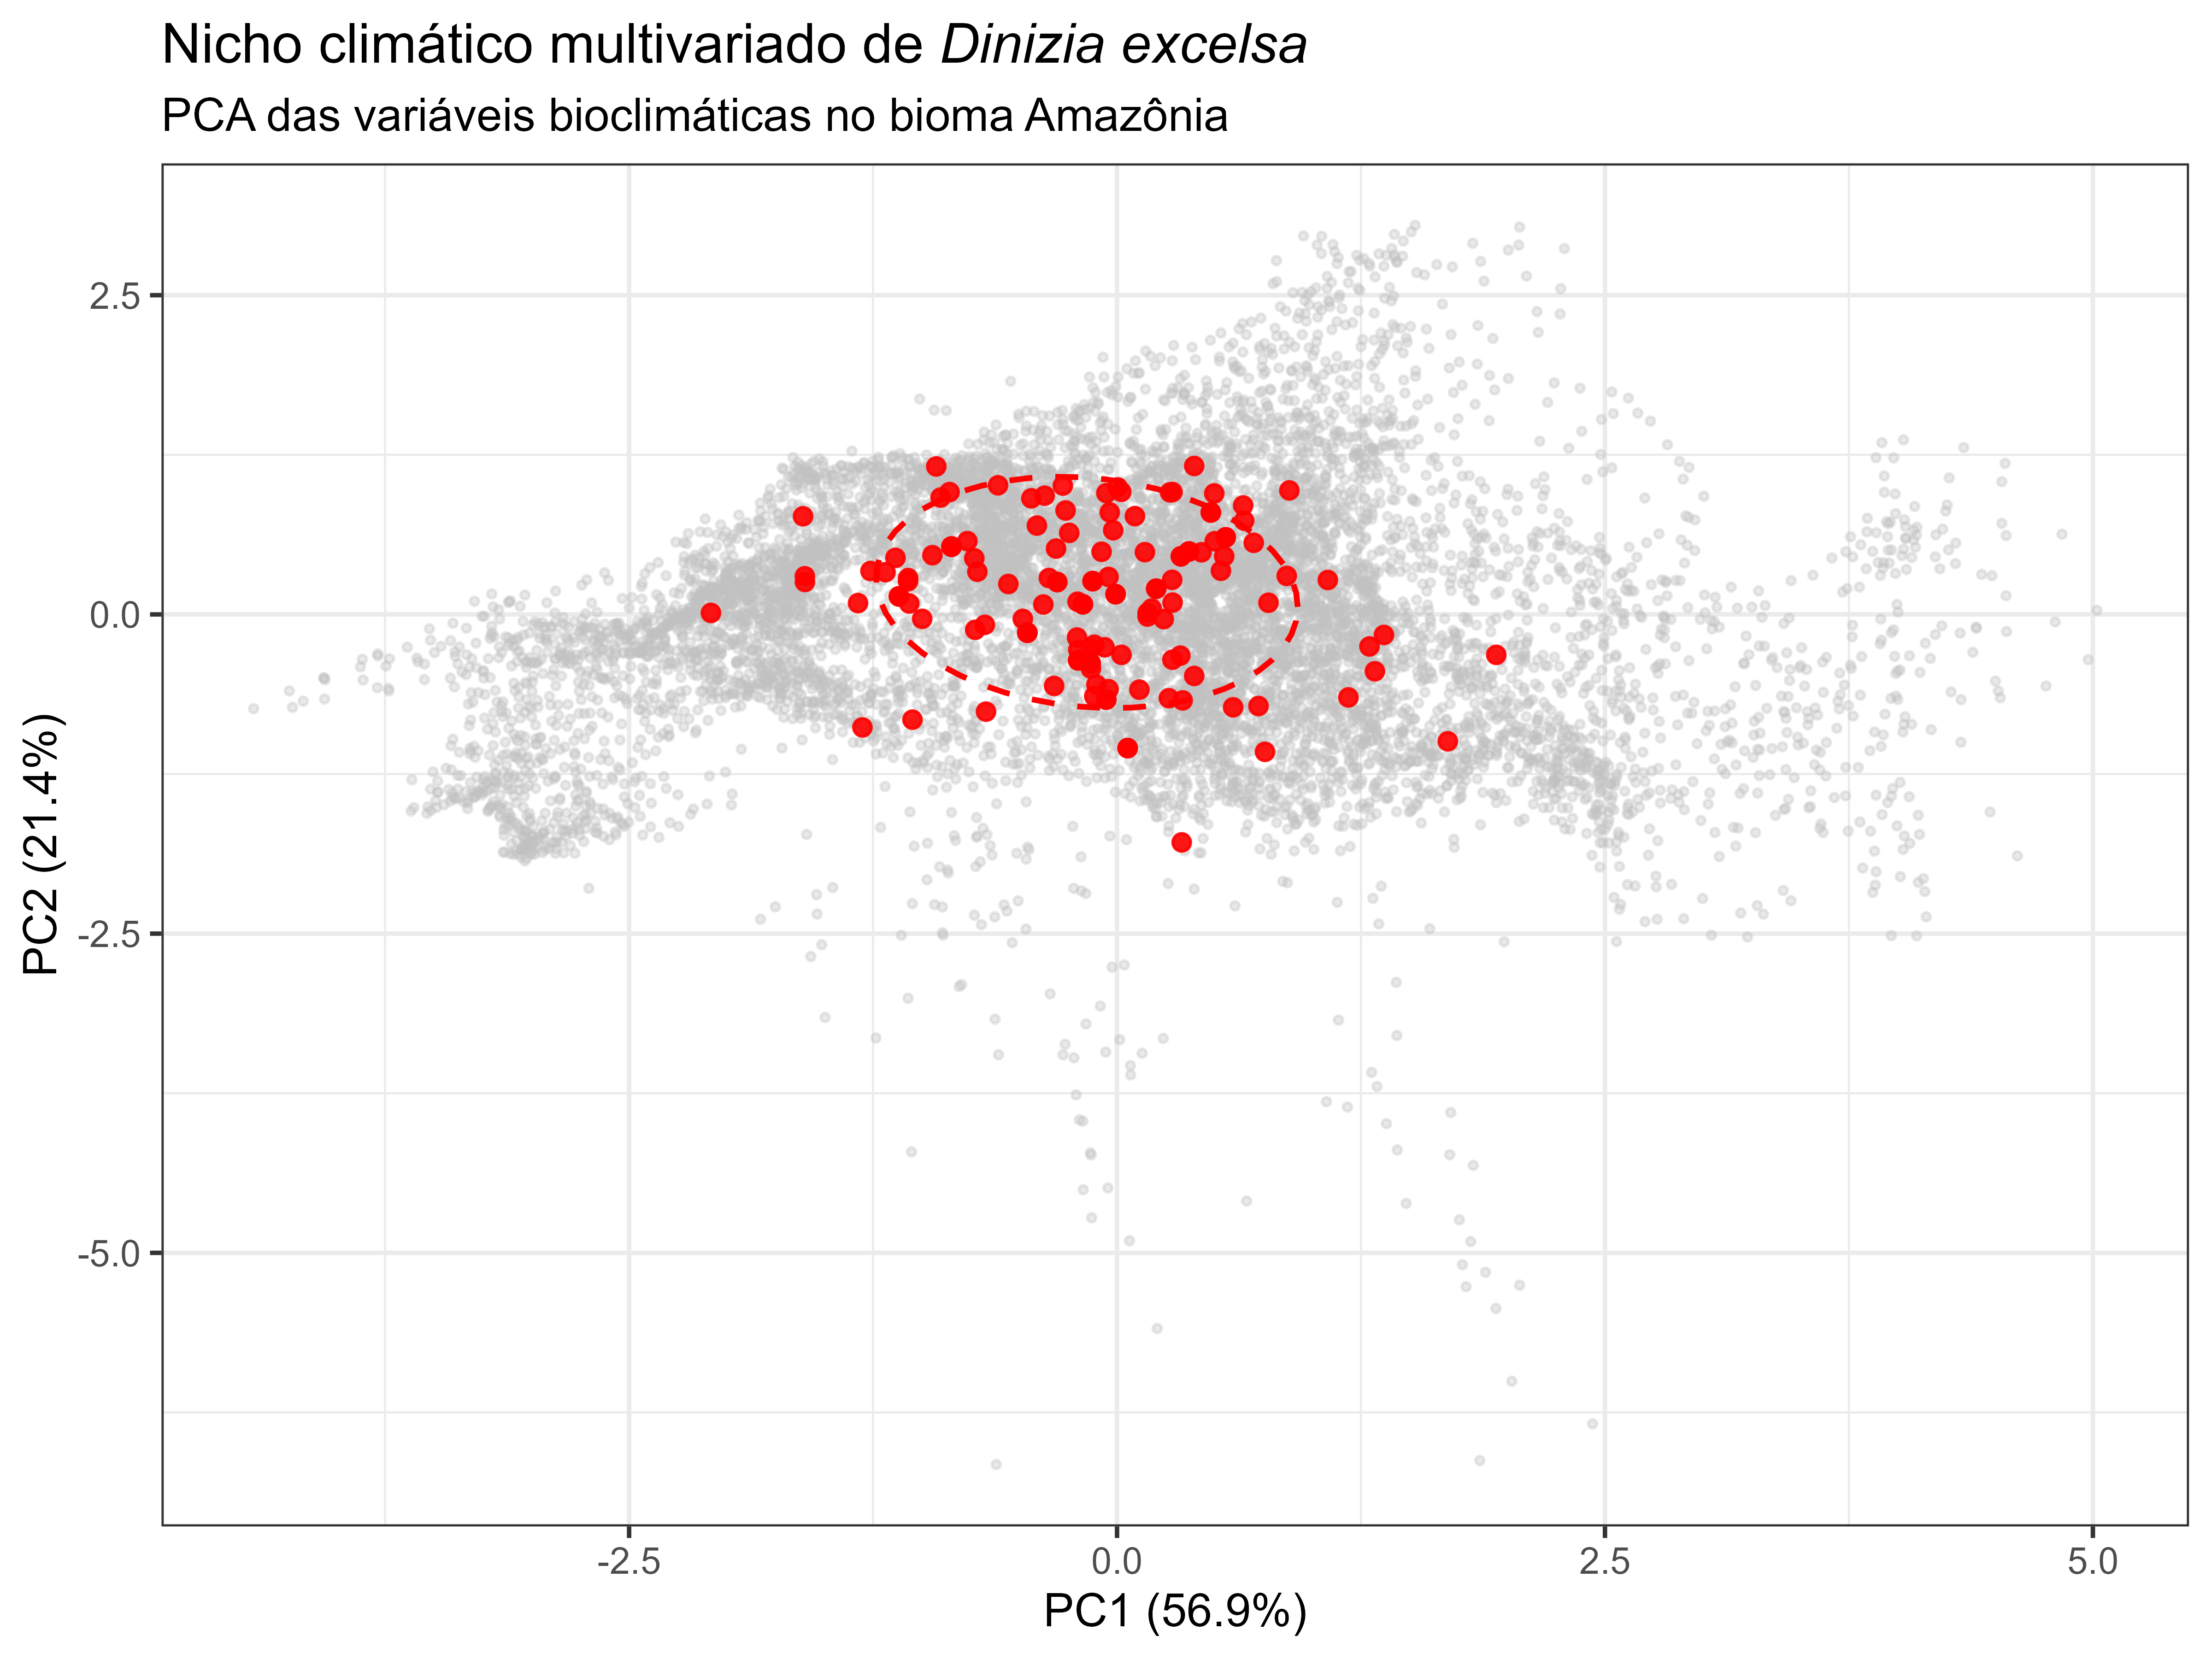
\includegraphics[width=0.82\textwidth]{figuras/unidade01/unidade01_pca_nicho_climatico_dinizia.png}
	\caption{Nicho climático multivariado de \textit{Dinizia excelsa} representado por PCA das variáveis bioclimáticas selecionadas. Os pontos cinza representam o background ambiental do bioma Amazônia e os pontos vermelhos representam as ocorrências da espécie.}
	\label{fig:unidade01_pca_dinizia}
\end{figure}

\begin{figure}[H]
	\centering
	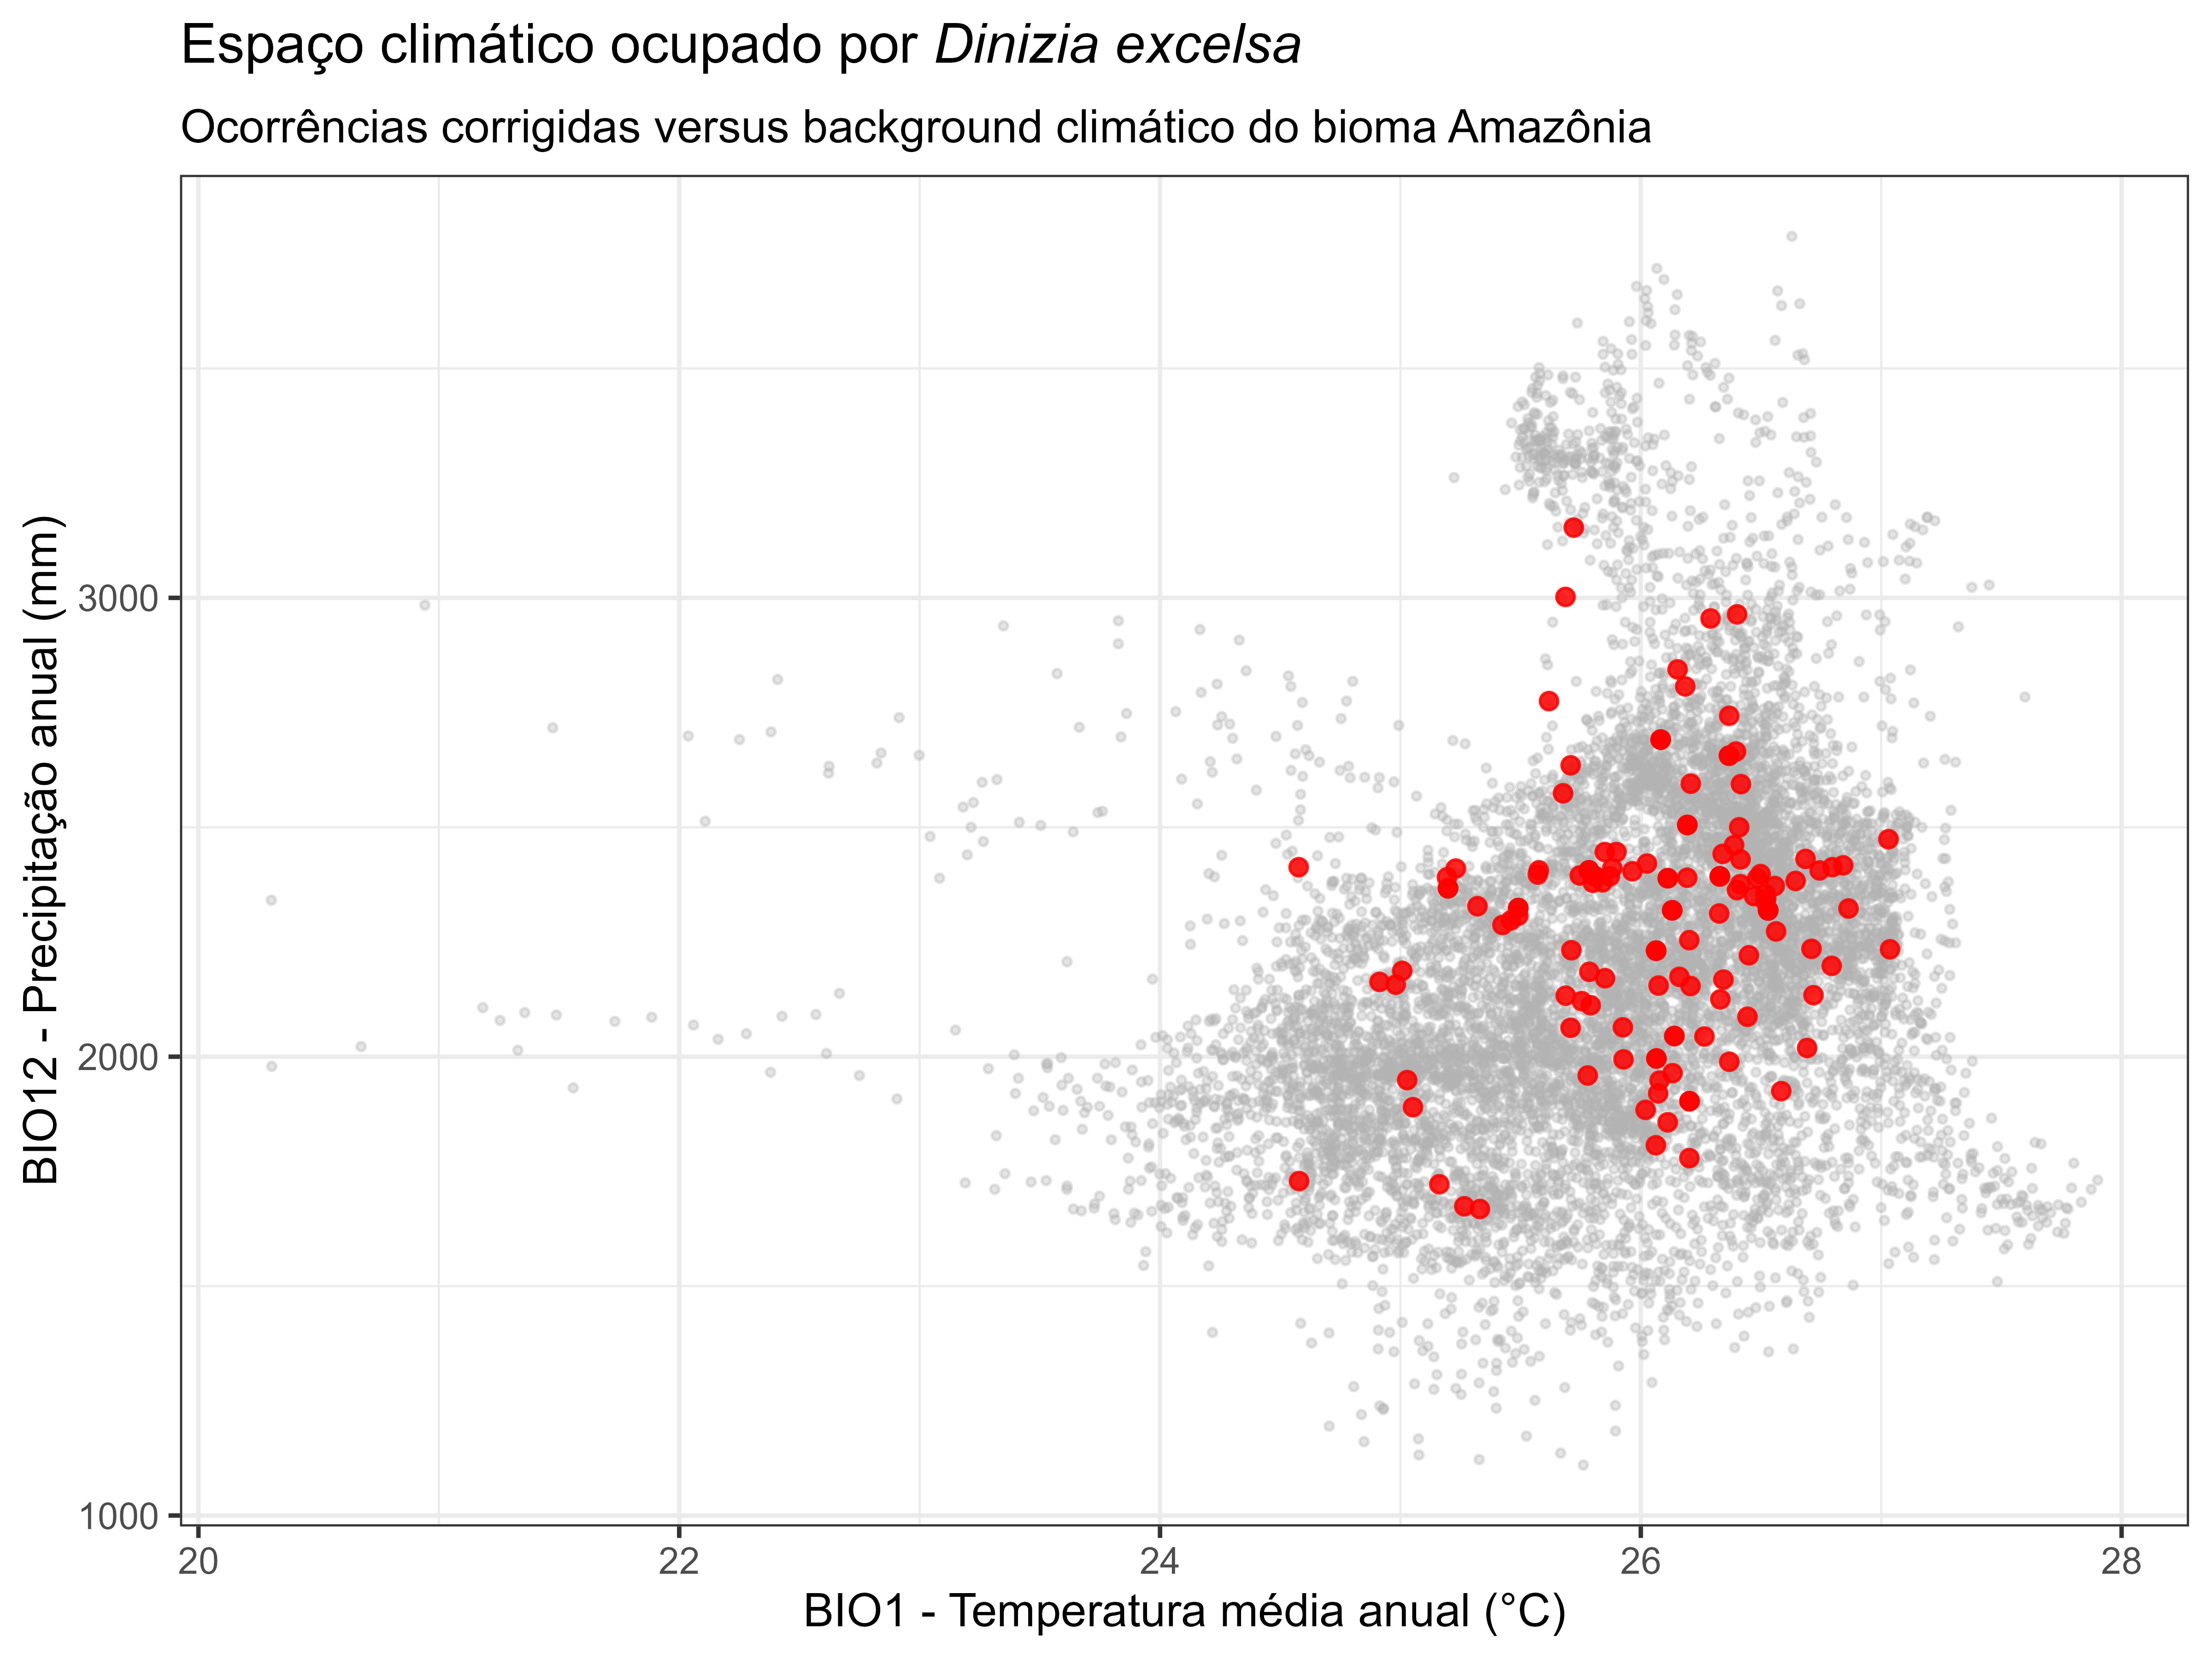
\includegraphics[width=0.82\textwidth]{figuras/unidade01/unidade01_nicho_temperatura_precipitacao_dinizia.png}
	\caption{Espaço climático ocupado por \textit{Dinizia excelsa} em relação ao background ambiental do bioma Amazônia, considerando temperatura média anual e precipitação anual.}
	\label{fig:unidade01_nicho_tp_dinizia}
\end{figure}

\begin{aplicacao}
	As Figuras~\ref{fig:unidade01_pca_dinizia} e~\ref{fig:unidade01_nicho_tp_dinizia} demonstram que a distribuição geográfica de \textit{Dinizia excelsa} está associada a um subconjunto específico das condições climáticas disponíveis no bioma Amazônia. O gráfico bivariado evidencia a ocupação do espaço climático definido pela temperatura média anual e pela precipitação anual, enquanto a PCA representa a posição da espécie em um espaço ambiental multidimensional construído a partir de múltiplas variáveis bioclimáticas. Observa-se que as ocorrências concentram-se em regiões ambientais relativamente mais restritas que o conjunto total de condições disponíveis no bioma, sugerindo processos de filtragem ecológica relacionados às exigências climáticas da espécie. Em estudos de Modelagem de Distribuição de Espécies, essas relações constituem a base para a estimativa do nicho ecológico e para a projeção de áreas potencialmente adequadas sob condições ambientais atuais, passadas ou futuras.
\end{aplicacao}

\begin{exercicios}
\begin{enumerate}
  \item Explique a diferença entre nicho de Grinnell, nicho de Elton e nicho de Hutchinson.
  \item Por que modelos de distribuição baseados em dados de ocorrência geralmente estimam uma aproximação do nicho realizado, e não do nicho fundamental?
  \item Diferencie distribuição observada, distribuição real e distribuição potencial.
  \item Explique por que ausência de registro em bases de biodiversidade não deve ser automaticamente interpretada como ausência ecológica da espécie.
  \item Discuta a importância da conservação de nicho para projeções climáticas futuras.
  \item Em espécies arbóreas amazônicas de grande porte, quais fatores podem fazer com que a distribuição de adultos não represente adequadamente a distribuição potencial de regenerantes?
\end{enumerate}
\end{exercicios}

% ============================================================
% UNIDADE 2
% ============================================================

